\documentclass[../main.tex]{subfiles}

\begin{document}
\section{Experiments -- Task3}

The model used here is a basic Artificial Neural Network with 12 dense layers,
using LeakyReLU as activation function. The output layer applies the sigmoid
function, with 1 representing full confidence in assigning the object to class 1, and 0
- full confidence in assigning it to 0.

Importantly for the plots seen later, this model also used the
$1-\mathrm{old\_value}$ trick for cost criteria. This was done to make the model
a more comparable to ANN-UTADIS (for the same reason, it has the same number of layers).

\subsection{Model visualization}
\begin{figure}[H]
    \centering
    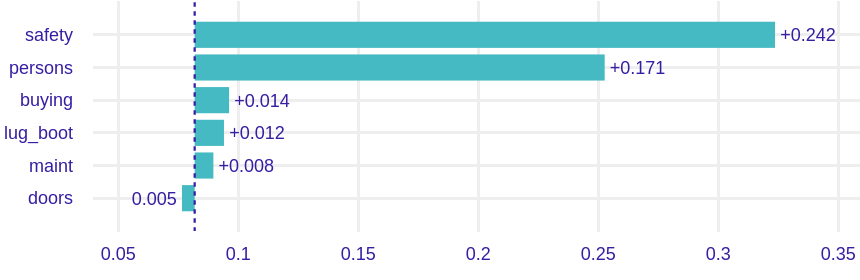
\includegraphics[width=\linewidth]{../img/ANN-feature-importance.png}
    \caption{ANN feature importance as computed by DALEX}
    \label{fig:ANN-feats}
\end{figure}

\subsection{Preference analysis}

The ANN model is essentially completely opaque. There are no explicit parameters
we could use to learn about DM's preferences.
However, the feature importance plot (and other visualizations, some of which are presented
later on in this report) can give us some insight:

- the order of feature importance is very similar to the one produced by ANN-UTADIS.
The only difference is "right-shifting" the 3rd, 4th and 5th most impactful features by 2
(UTA: \emph{maint}>\emph{buying}>\emph{lug\_boot}; ANN: \emph{buying}>\emph{lug\_boot}>\emph{maint})

- \emph{safety} and \emph{persons} dominate other features in terms of assigned importance

- very interestingly, \emph{door} is completely irrelevant or even counterproductive. This is
a clear example of how a black box model can learn something that makes no sense in the real world.

A fun way to summarise this picture, is to think that the model created an image of someone
looking to buy a bus - a safe vehicle, capable of carrying many passengers, and one they are
unlikely to have to pay for on their own. Low priority on \emph{lug\_boot} still makes sense,
as well as not really caring about the number of doors - a tourist coach can do fine with one,
and it might make counting passengers, or collecting payments from them easier.

\subsection{3-alternative analysis}

\subsubsection{Analytical approach}

There is no way to analytically give any estimates on how the output would change,
as the created neural network has too many parameters interacting in too complex
ways for a human to reasonably handle. The only thing that can be said for certain
is that making the same change for \emph{mid} as in ANN-UTADIS (setting \emph{doors}=0.25)
would not result in the model deeming it acceptable.

I would wager that similarly as in ANN-UTADIS, changing just a single parameter would not
be enough to change the classification of the \emph{best} and \emph{worst} alternatives.
However, since \emph{mid} has a \emph{safety} of 0, and this is the most impactful attribute,
there probably exists a threshold on it that if \emph{mid} were to exceed, it
would make the model change its mind on this alternative's classification.
This threshold is probably at least in the neighbourhood of 0.25, but I have no confidence
in making more precise guesses.

\subsubsection{Space sampling}
To concisely show how changing the value of just one attribute would change the result, ceteris paribus analysis
was performed.
Files with all plots are available in \verb|report/img/extras|. In order not to overcrowd the report,
only the plots for \emph{safety} for the 3 alternatives are presented.

\begin{figure}
    \centering
    \begin{subfigure}[b]{0.48\linewidth}
        \makeatletter\def\@currentlabel{DALEX plot}\makeatother
        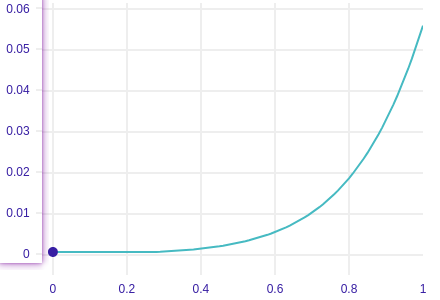
\includegraphics[width=\linewidth]{../img/ANN_safety_worst.png}
        \label{fig:ANN-ceteris-paribus-safety}
    \end{subfigure}
    \begin{subfigure}[b]{0.48\linewidth}
        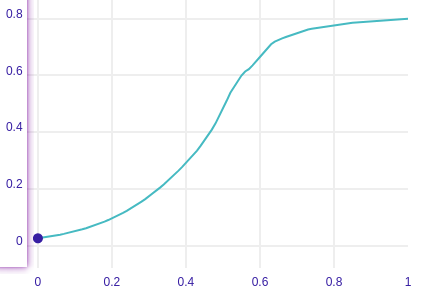
\includegraphics[width=\linewidth]{../img/ANN_safety_mid.png}
    \end{subfigure}

    \begin{subfigure}[b]{0.48\linewidth}
        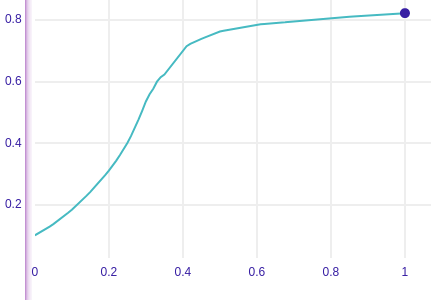
\includegraphics[width=\linewidth]{../img/ANN_safety_best.png}
    \end{subfigure}

    \caption{Ceteris paribus analysis for criterion \emph{safety} for (in order, from left to right and
    top to bottom): \emph{worst}, \emph{mid}, \emph{best}}
\end{figure}

These plots suggest, that to make \emph{mid} acceptable, setting safety to around
0.5 would be necessary. No amount of change on any other attribute would make \emph{mid} acceptable.

\subsubsection{Variable contribution plots}
\begin{figure}[H]
    \centering
    \begin{subfigure}{\linewidth}
        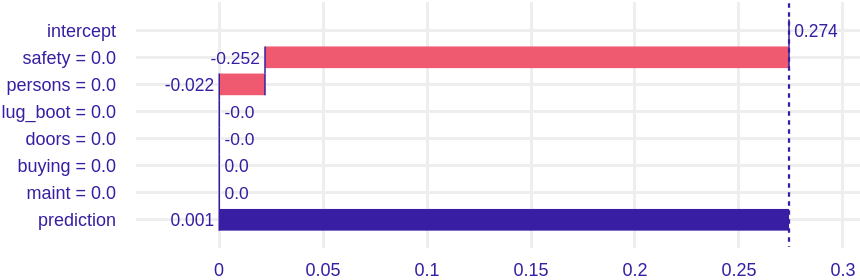
\includegraphics[width=\linewidth]{../img/ANN-breakdown-worst.png}
        \caption{Variable contribution of alternative 1 (worst) in ANN}
        \label{fig:ANN-3alt1-contrib}
    \end{subfigure}
    \begin{subfigure}{\linewidth}
        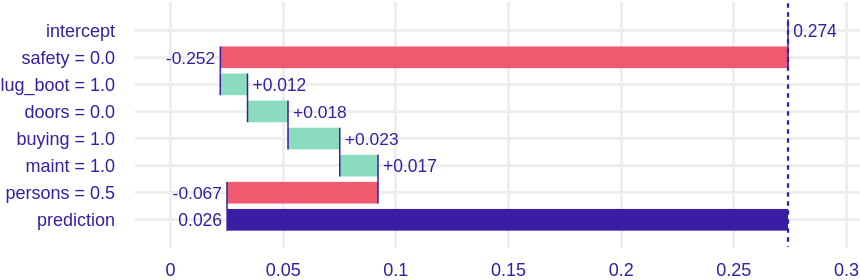
\includegraphics[width=\linewidth]{../img/ANN-breakdown-mid.png}
        \caption{Variable contribution of alternative 2 (mid) in ANN}
        \label{fig:ANN-3alt2-contrib}
    \end{subfigure}
    \begin{subfigure}{\linewidth}
        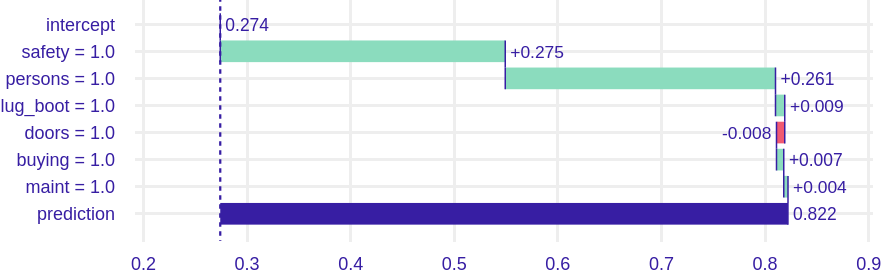
\includegraphics[width=\linewidth]{../img/ANN-breakdown-best.png}
        \caption{Variable contribution of alternative 3 (best) in ANN}
        \label{fig:ANN-3alt3-contrib}
    \end{subfigure}
\end{figure}

\end{document}
